\section{Discussion}
\label{sec:discussion}

We have presented CHAODA, an ensemble of four algorithms that use the map of the underlying manifold produced by CLAM\@.
The four individual algorithms are simple to implement on top of CLAM and, when combined into an ensemble, often outperform the state-of-the-art in anomaly detection.

CLAM uses the geometric and topological properties of fractal dimension and metric entropy of the data to build a map of the low-dimensional manifold that the data occupy.
CLAM builds on the clustering algorithm from CHESS~\cite{ishaq2019clustered}, adding a novel graph-induction approach and a notion of optimal depths, learned via a form of ``meta-machine-learning'' and transfer learning.
CHAODA builds on this manifold-mapping framework for anomaly and outlier detection.
Intuitively, we expect CHAODA to perform particularly well when the data lie on an ``interesting'' manifold, and to perform merely average when the data derive from an easily-described distribution (or ``boring'' manifold).
Just as CHESS demonstrated an acceleration of search when the data exhibited \emph{low fractal dimension} and \emph{low metric entropy}, with CHAODA, we see that AUC scores are vastly improved when the data exhibit these properties and are often competitive when the data do not exhibit these properties.

% A simple visualization in Figure~\ref{fig:conclusions:umap-embeddings} using UMAP~\cite{mcinnes2018umap} illustrates two different examples; the anomalies in one dataset appear to be at the edges of the manifold (though, clearly, the UMAP projection has distorted the manifold) while in another datset they appear distributed along the less-interesting distribution.

% TODO choose two different datasets, not to illustrate performance but to illustrate this point!

% Except for the annthyroid dataset, the algorithms presented here outperform or at least nearly match all other approaches.
% CHAODA outperforms a 1-class SVM on every dataset, and of the datasets where AUC values were available for other results (20 datasets), CHAODA matches or exceeds the AUC of other approaches on 12 of them.
% On 5 of the remaining 8, CHAODA is close to the best-performing approach, typically within 1 and 3 percentage points.

% Several reasons may contribute to CHAODA's difficulty with the annthyroid dataset in particular.
% First, this dataset was specifically created for use with ANNs.
% Upon further investigation, it appears that these data may be in too few dimensions for CLAM to partition it into a useful manifold.
% In UMAP~\cite{mcinnes2018umap} projections we created on annthyroid Figure~\ref{fig:conclusions:umap-embeddings}, it can be clearly seen that the anomalous data appear to live directly on the manifold, with only a small pocket appearing to be distinctly off.
% In contrast, the wbc dataset, where CHAODA significantly outperforms HiCS~\cite{keller2012hics}, appears to have most of the outliers along the periphery of the manifold.
% This aligns well with our expectations of CHAODA\@.
% Indeed, the manifold being both learnable and distinctly separate from the anomalous data are mandatory properties for any of our approaches to be effective.
% Fortunately, we can see that these properties are apparent in all other datasets studied.

% \begin{figure*}
%    \centering
%    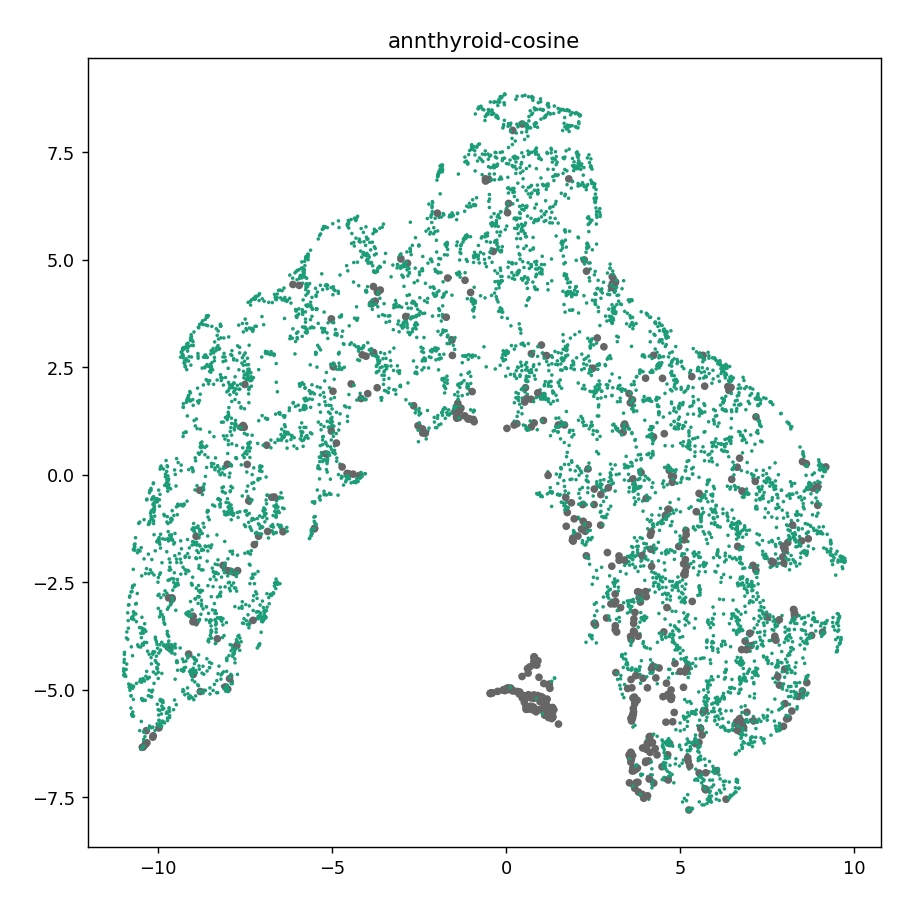
\includegraphics[width=2in]{images/umaps/annthyroid-cosine-umap2d.png}
%    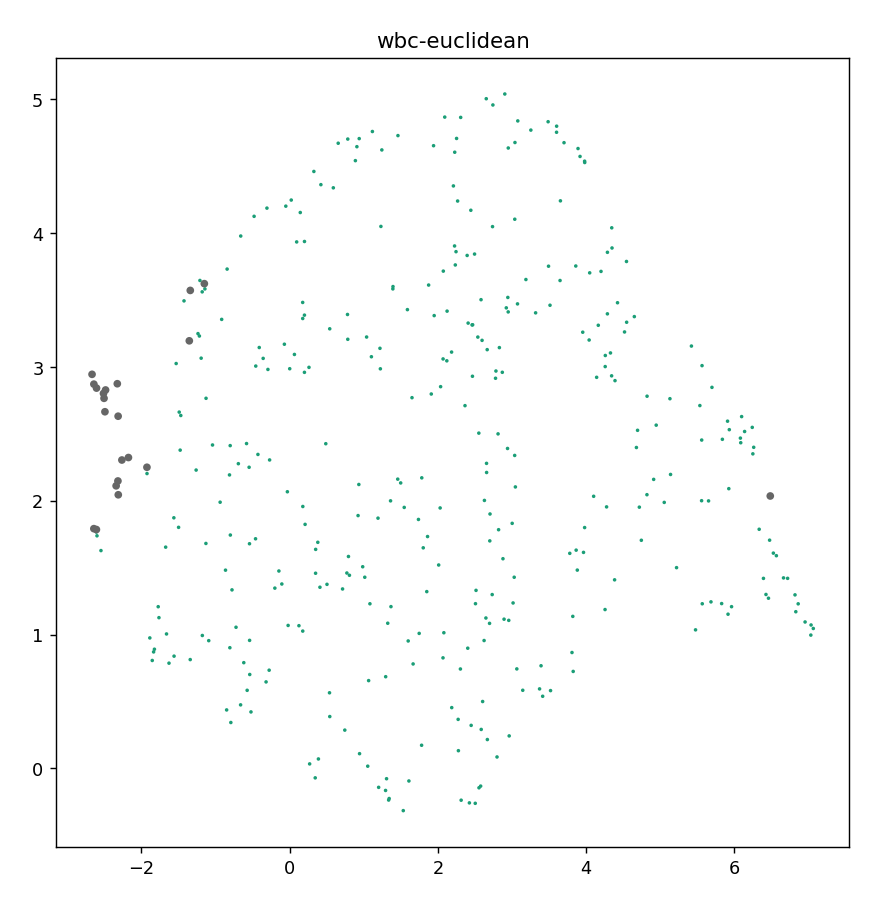
\includegraphics[width=2in]{images/umaps/wbc-euclidean-umap2d.png}
%    \caption{UMAP projection of Annthyroid (left) and WBC (right). Anomalies are in gray. Note that for Annthyroid, while there is a cluster of anomalies off the main manifold, many anomalies are distributed throughout the manifold. For WBC, the anomalies tend to be at the edge of the manifold.}
%    \label{fig:conclusions:umap-embeddings}
% \end{figure*}

% \subsection{Future Directions}
% \label{subsec:discussion:duture-directions}

The choice of distance function seems to have a significant impact on anomaly-detection performance.
In this case, domain knowledge is likely the best way to determine the distance function of choice.
Future work should explore a more diverse collection of domain-appropriate distance functions, such as Wasserstein distance on images, Levenshtein edit distance on strings, and Jaccard Index on the Maximal Common Sub-Graph of molecular structures.

Since CHAODA is highly effective on high-dimensional datasets, we can apply it to study Neural Networks.
We can create a dataset where each datum represents the activations of a neural network from an input to the neural network.
After mapping the manifold of such activations, we would expect to detect malicious inputs to neural networks based on the intuition that malicious inputs produce atypical activation patterns.

% \subsection{Conclusion}
% \label{subsec:discussion:conlcusion}

In conclusion, we have demonstrated that by mapping the manifolds occupied by data, we can exploit that knowledge to implement simple algorithms capable of outperforming other state-of-the-art approaches to anomaly detection.

% TODO discuss runtime
